\documentclass[12pt,a4paper,notitlepage]{report}
\usepackage[utf8]{inputenc}
\usepackage[polish]{babel}
\usepackage[T1]{fontenc}
\usepackage[top=2cm, bottom=2cm, left=3cm, right=3cm]{geometry}
\usepackage[dvipsnames]{xcolor}
\definecolor{Red}{RGB}{255,36,0}
\usepackage{changepage}
\usepackage{indentfirst}
\usepackage{color}
\usepackage{graphicx}
\definecolor{bluekeywords}{rgb}{0.13,0.13,1}
\definecolor{greencomments}{rgb}{0,0.5,0}
\definecolor{redstrings}{rgb}{0.9,0,0}
\usepackage{listings}
\lstset{language=[Sharp]C,
  showspaces=false,
  showtabs=false,
  breaklines=true,
  showstringspaces=false,
  breakatwhitespace=true,
  escapeinside={(*@}{@*)},
  commentstyle=\color{greencomments},
  keywordstyle=\color{bluekeywords},
  stringstyle=\color{redstrings},
  basicstyle=\ttfamily,
  extendedchars=true
}
\makeatletter
\newcommand{\linia}{\rule{\linewidth}{0.4mm}}
\renewcommand{\maketitle}{\begin{titlepage}
    \vspace*{1cm}
    \begin{center}\small
    Politechnika Wrocławska\\
    Wydział Elektroniki\\
    Urządzenia Peryferyjne 
    \end{center}
    \vspace{4.5cm}
    \noindent\linia
    \begin{center}
      \LARGE \textsc{\@title}
         \end{center}
     \linia
    \vspace{0.5cm}
    \begin{flushright}
    \begin{minipage}{6cm}
    
     \vspace{4cm}
     \textit{\small Termin zajęć:}\\
     \normalsize \textsc{Wtorek TN 7:30} \par
	\vspace{0.3cm}    
    \textit{\small Autorzy:}\\
    \normalsize \textsc{\@author} \par
     \vspace{0.3cm}
        Prowadzący: \\ dr inż. Tomasz Walkowiak

    \end{minipage}
    \vspace{1cm}
     {\small }\\
       
     \end{flushright}
    \vspace*{\stretch{3}}
    \begin{center}
    \@date
    \end{center}
  \end{titlepage}%
}
\makeatother
\author{ Jakub Chmiel  235028 \\ Tomasz Cieślar 235652}
\title{Obsługa skanera płaskiego (WIA 2.0)}
\begin{document}
\maketitle

\newpage
\tableofcontents
\newpage
\renewcommand*\thesection{\arabic{section}}
\section{Cel ćwiczenia}
\begin{enumerate}
\item Sprawdź czy skaner działa poprawnie
\item Napisać program wykonujący skanowanie przy pomocy skanera płaskiego.\\Możliwości programu obejmują:
\begin{itemize}
\item skanowanie z wykorzystaniem  UI
\item skanowanie bez wykorzystania  UI
\item wyświetlanie uzyskanego obrazu
\item zmiana trybu skanowania (1-bitowy, skala szarości, RGB)
\end{itemize}
\item Rozszerzyć działanie programu:
\begin{itemize}
\item zapis skanowanych obrazów do plików graficznych
\end{itemize}
\end{enumerate}

\section{Wstęp}
Windows Image Acquisition (WIA) jest platrformą do przechwytywania obrazów w systemach operacyjnych z rodziny Windows, począwszy od Windowsa Millenium Edition i Windowsa XP.
\\
\indent Platforma WIA pozwala na interakcję między aplikacjami a sprzętem do przechwytywania obrazów i standaryzuje interakcje między różnymi aplikacjami a skanerami. Pozwala to różnym aplikacjom na porozumiewanie się z różnymi skanerami bez konieczności modyfikowania aplikacji przez programistów i sterowników przez producentów skanerów dla każdej kombinacji sprzętu i programów.

\section{Założenia projektowe}
\begin{itemize}
\item Program był pisany w języku C\texttt{\#}.
\item Na komputerze, na którym uruchamiany był program zainstalowano system operacyjny Windows 10 w wersji 64-bitowej.
\end{itemize}

\section{Wykorzystane narzędzia}
\begin{itemize}
\item Windows Forms - API do implementacji interfejsu graficznego dla platformy .NET.
\item WIA 2.0 - aktualna wersja platformy WIA, po raz pierwszy wprowadzona w systemie Windows Vista.
\end{itemize}
\begin{adjustwidth}{0pt}{-50pt}
\section{Implementacja programu}
\subsection{Interfejs aplikacji}
\noindent 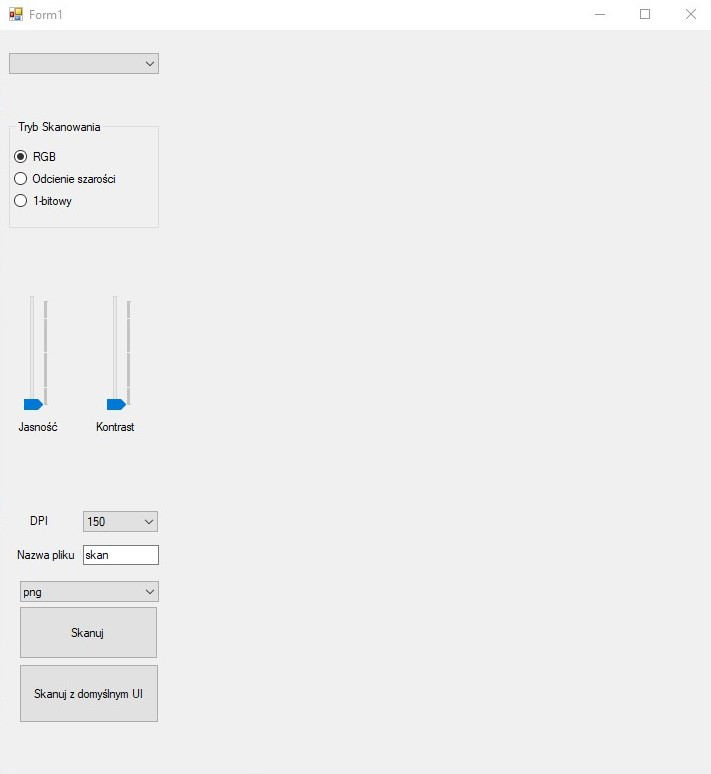
\includegraphics[scale=0.85]{okno}
\begin{center}
\begin{normalsize}
\textit{Rysunek 1. Interfejs aplikacji}
\end{normalsize}
\end{center}
\newpage
\subsection{Kod źródłowy}
\subsubsection{Okno aplikacji}
\begin{lstlisting}
using [...]

namespace UP_Skaner
{
    public partial class Form1 : Form
    {
        private ScannerClass device;

        public Form1()
        {
            InitializeComponent();
            ListDevices();
            device = (ScannerClass)comboBox2.SelectedItem;
        }

		//wylistowanie wszystkich urzadzen
        public void ListDevices()
        {
            var deviceManager = new DeviceManager();

            for (int i = 1; i <= deviceManager.DeviceInfos.Count; i++)
            {
            	//zebranie wszystkich urzadzen typu skaner
                if (deviceManager.DeviceInfos[i].Type == WiaDeviceType.ScannerDeviceType)
                {
                    comboBox2.Items.Add(new ScannerClass(deviceManager. DeviceInfos[i]));
                }
            }
        }

        private void comboBox2_SelectedIndexChanged(object sender, EventArgs e)
        {
            device = (ScannerClass)comboBox2.SelectedItem;
        }
        
        private void button1_Click(object sender, EventArgs e)
        {
            //wyczyszczenie podgladu
            pictureBox1.Image = null;
            if (device != null)
            {
                var connectedDevice = device._deviceInfo.Connect();
                var scannerItem = connectedDevice.Items[1];

                ImageFile image;
                //ustawienie trybu koloru
                if (radioButton1.Checked)
                    SetColorMode(scannerItem, 1);
                else if(radioButton2.Checked)
                {
                    SetColorMode(scannerItem, 2);
                }
                else if (radioButton3.Checked)
                {
                    SetColorMode(scannerItem, 4);
                }

		//ustawienie DPI
                int dpi = Int32.Parse(comboBox3.Text);
                SetDPI(scannerItem, dpi);
                
                //ustawienie rozmiaru
                SetHeightWidth(scannerItem,1250,1700);
				
		//ustawienie jasnosci
                SetBrightness(scannerItem, trackBar1.Value);
                
                //ustawienie kontrastu
                SetContrast(scannerItem, trackBar2.Value);

		//rozszerzenia zapisanego pliku
                switch (comboBox1.SelectedItem)
                {
                    case "png":
                        image = (ImageFile) scannerItem.Transfer (FormatID.wiaFormatPNG);
                        break;
                    case "jpeg":
                        image = (ImageFile)scannerItem.Transfer (FormatID.wiaFormatJPEG);
                        break;
                    case "tiff":
                        image = (ImageFile)scannerItem.Transfer (FormatID.wiaFormatTIFF);
                        break;
                    default:
                        image = (ImageFile)scannerItem.Transfer (FormatID.wiaFormatJPEG);
                        break;
                }
				
		//ustawienie nazwy pliku
                var path = $"{textBox1.Text}.{comboBox1.SelectedItem}";
				
				
		//usuniecie pliku jesli istnieje
                if (File.Exists(path))
                {
                    File.Delete(path);
                }
				
		//zapisanie pliku
                image.SaveFile(path);
                
                //ustawienie obrazu jako podglad
                pictureBox1.Image = new Bitmap(path);
                pictureBox1.SizeMode = PictureBoxSizeMode.StretchImage;
            }
            else
            {
                MessageBox.Show("Wybierz urzadzenie");
            }
        }
		
	//stale biblioteki WIA
        const string WIA_SCAN_COLOR_MODE = "6146";
        const string WIA_HORIZONTAL_SCAN_RESOLUTION_DPI = "6147";
        const string WIA_VERTICAL_SCAN_RESOLUTION_DPI = "6148";

        const string WIA_HORIZONTAL_SCAN_START_PIXEL = "6149";
        const string WIA_VERTICAL_SCAN_START_PIXEL = "6150";

        const string WIA_HORIZONTAL_SCAN_SIZE_PIXELS = "6151";
        const string WIA_VERTICAL_SCAN_SIZE_PIXELS = "6152";

        const string WIA_SCAN_BRIGHTNESS_PERCENTS = "6154";
        const string WIA_SCAN_CONTRAST_PERCENTS = "6155";
       
       //ustawienie trybu kolorow
        public void SetColorMode(IItem scannerItem, int mode)
        {
            SetWIAProperty(scannerItem.Properties, WIA_SCAN_COLOR_MODE, mode );
        }
		
		
		
	//ustawienie rozmiarow obrazu
        public void SetHeightWidth(IItem scannerItem, int width, int height)
        {
            SetWIAProperty(scannerItem.Properties, WIA_HORIZONTAL_SCAN_SIZE_PIXELS, width);
            SetWIAProperty(scannerItem.Properties, WIA_VERTICAL_SCAN_SIZE_PIXELS, height);
        }

	//ustawienie DPI
        public void SetDPI(IItem scannerItem, int dpi)
        {
            SetWIAProperty(scannerItem.Properties, WIA_HORIZONTAL_SCAN_RESOLUTION_DPI, dpi);
            SetWIAProperty(scannerItem.Properties, WIA_VERTICAL_SCAN_RESOLUTION_DPI, dpi);
        }

	//ustawienie parametru w bibliotece WIA
        private static void SetWIAProperty(IProperties props, object propName, object propValue)
        {
            Property property = props.get_Item(ref propName);
            property.set_Value(ref propValue);
        }

	//ustawienie jasnosci
        public void SetBrightness(IItem scannerItem, int value)
        {
            SetWIAProperty(scannerItem.Properties, WIA_SCAN_BRIGHTNESS_PERCENTS, value);
        }

	//ustawienie kontrastu
        public void SetContrast(IItem scannerItem, int value)
        {
            SetWIAProperty(scannerItem.Properties, WIA_SCAN_CONTRAST_PERCENTS, value);
        }

	//skanowanie z domyslnym UI
        private void button2_Click(object sender, EventArgs e)
        {
            //format JPEG
            const string wiaFormatJPEG = "{B96B3CAE-0728-11D3-9D7B-0000F81EF32E}";
            //nazwa pliku
            String fileName = "skan_bez_UI";
            
            //CommonDIalog - domyslne okno skanowania systemu Windows
            ICommonDialog wiaDiag = new WIA.CommonDialog();
            ImageFile wiaImage = null;
            //pobranie obrazu z okreslonymi ustawieniami
            wiaImage = wiaDiag.ShowAcquireImage(WiaDeviceType. UnspecifiedDeviceType, WiaImageIntent.GrayscaleIntent, WiaImageBias.MaximizeQuality,
                wiaFormatJPEG, true, true, false);
            Vector vector = wiaImage.FileData;
            //ustawienie podgladu
            pictureBox1.Image = Image.FromStream(new MemoryStream((byte[])vector.get_BinaryData()));
	    //stworzenie obrazu
            Image img = Image.FromStream(new MemoryStream((byte[])vector.get_BinaryData()));
            zapis obrazu
            img.Save(fileName + ".JPEG");
        }
    }
}
\end{lstlisting}
\subsubsection{Klasa ScannerClass}
\begin{lstlisting}
using [...]

namespace scanner
{
    //Klasa pomocnicza. Jej funkcja jest poprawne wypelnienie ComboBoxa do wyboru skanera
    class ScannerClass
    {
        public DeviceInfo _deviceInfo;
        public ScannerClass(DeviceInfo info)
        {
            _deviceInfo = info;
        }

        public override string ToString()
        {
            return (string)_deviceInfo.Properties["Name"]. get_Value();
        }
    }
}
\end{lstlisting}

\end{adjustwidth}
\newpage
\section{Wnioski}
Podczas ćwiczenia poznaliśmy podstawową obsługę skanera i funkcje takie jak zmiana parametrów skanowania, zapis do pliku, podgląd, czy wywołanie domyślnego interfejsu systemu Windows. Biblioteka WIA 2.0 okazała się intuicyjna w użyciu i pozwoliła na sprawne wykonanie zadań.
\section{Bibliografia}
\begin{itemize}
\item Dokumentacja Microsoftu:
\\
$https://docs.microsoft.com/en-us/windows/desktop/wia/-wia-startpage$
\end{itemize}

\end{document}